\documentclass{article}
\usepackage{amsmath}
\usepackage{amsthm}
\usepackage{amsfonts}
\usepackage{amssymb}
\usepackage{bbold}
\usepackage{dsfont}
\usepackage{graphicx}
\usepackage{cleveref}
\usepackage{bm}
\usepackage{booktabs}
\usepackage{siunitx}
\usepackage{xcolor}
\usepackage{pdfpages}
\usepackage[utf8]{inputenc}
\usepackage[english]{babel}
\newtheorem{definition}{Definition}
\newtheorem{example}{Example}
\newcommand{\exP}[1]{\mathrm{e}^{#1}}
\newcommand{\dif}{\mathrm{d}}
\renewcommand{\vec}[1]{\mathbf{#1}}
\newcommand{\pdagger}{{\phantom{\dagger}}}
\newcommand{\state}[1]{\vert #1\rangle}
\newcommand{\cstate}[1]{\langle #1\vert}
\newcommand{\tr}[1]{\mathrm{tr}\left\{#1\right\}}
\newcommand{\trs}[2]{\, \mathrm{tr}_{#1}\{#2\}}
\newcommand{\expc}[3]{\langle #1\vert #2 \vert #3\rangle}
\usepackage[doi=false,url=false,isbn=false,backend=bibtex,style=nature,natbib=true,sorting=none]{biblatex}
\bibliography{bib.bib}
\usepackage{geometry}
\geometry{
	a4paper,
	total={170mm,257mm},
	left=15mm,
	right=15mm,
	top=15mm,
}
\begin{document}
\title{Report 29: Non-interacting system with TT-HEOM}
\maketitle
\section{Model}
The following tests are for the model introduced in \cite{fransson2019chirality}, which is without vibrational modes, and reads
\begin{align}
			H &= H_\mathrm{mol} +   H_\mathrm{leads}+H_\mathrm{mol-leads},
\end{align}
	\begin{align}
	H_\mathrm{mol} &=
	\begin{aligned}[t]
		&\sum_{j\sigma} \varepsilon_{0}^\pdagger d_{j\sigma}^\dagger d_{j\sigma}^\pdagger -  \sum_{j\sigma} t_0^\pdagger (d_{j\sigma}^\dagger d_{j+1,\sigma}^\pdagger + \mathrm{h.c.})+\\
		& \sum_{j\sigma\sigma'} \lambda_0^\pdagger(id_{j\sigma}^\dagger (\vec{v}_j^{(+)}\cdot \bm{\sigma})_{\sigma\sigma'}^\pdagger d_{j+2,\sigma'}^\pdagger + \mathrm{h.c.})+\\
		& \sum_j U  d_{j\uparrow}^\dagger d_{j\uparrow}^\pdagger d_{j\downarrow}^\dagger d_{j\downarrow}^\pdagger,
	\end{aligned}
	\label{eq:H_el}\\[\jot]
\end{align}
	\begin{align}
	H_\mathrm{leads} = \sum_{\ell \in \{L,R\}} \sum_{\alpha,\sigma} \varepsilon_{\ell \alpha \sigma}^\pdagger c_{ \ell \alpha \sigma}^\dagger c_{\ell \alpha \sigma}^\pdagger,
\end{align}
\begin{align}
	H_{\mathrm{mol}-\mathrm{leads}} = 
	&\sum_{\alpha, \sigma} \big(\gamma_{L \alpha \sigma}^\pdagger d_{1\sigma}^\dagger c_{L \alpha \sigma}^\pdagger + \gamma_{R \alpha \sigma}^\pdagger d_{N\sigma}^\dagger c_{R \alpha \sigma}^\pdagger+\mathrm{h.c.}\big)
\end{align}
\section{Parameters}
Parameters taken from \cite{fransson2019chirality}
\begin{align*}
	\Gamma&=\SI{10}{\milli\electronvolt}\\
	t_0&=\SI{40}{\milli\electronvolt}\\
	\varepsilon_0&= -\SI{300}{\milli\electronvolt}\\
	\lambda_0 &= \SI{5}{\milli\electronvolt}\\
	\Phi &= \SI{600}{\milli\volt}\\
	k_BT &=\SI{25}{\milli\electronvolt}.
\end{align*}
\clearpage
\section{Comparison of ranks for varying system size}
\begin{figure}[!h]
	\centering
	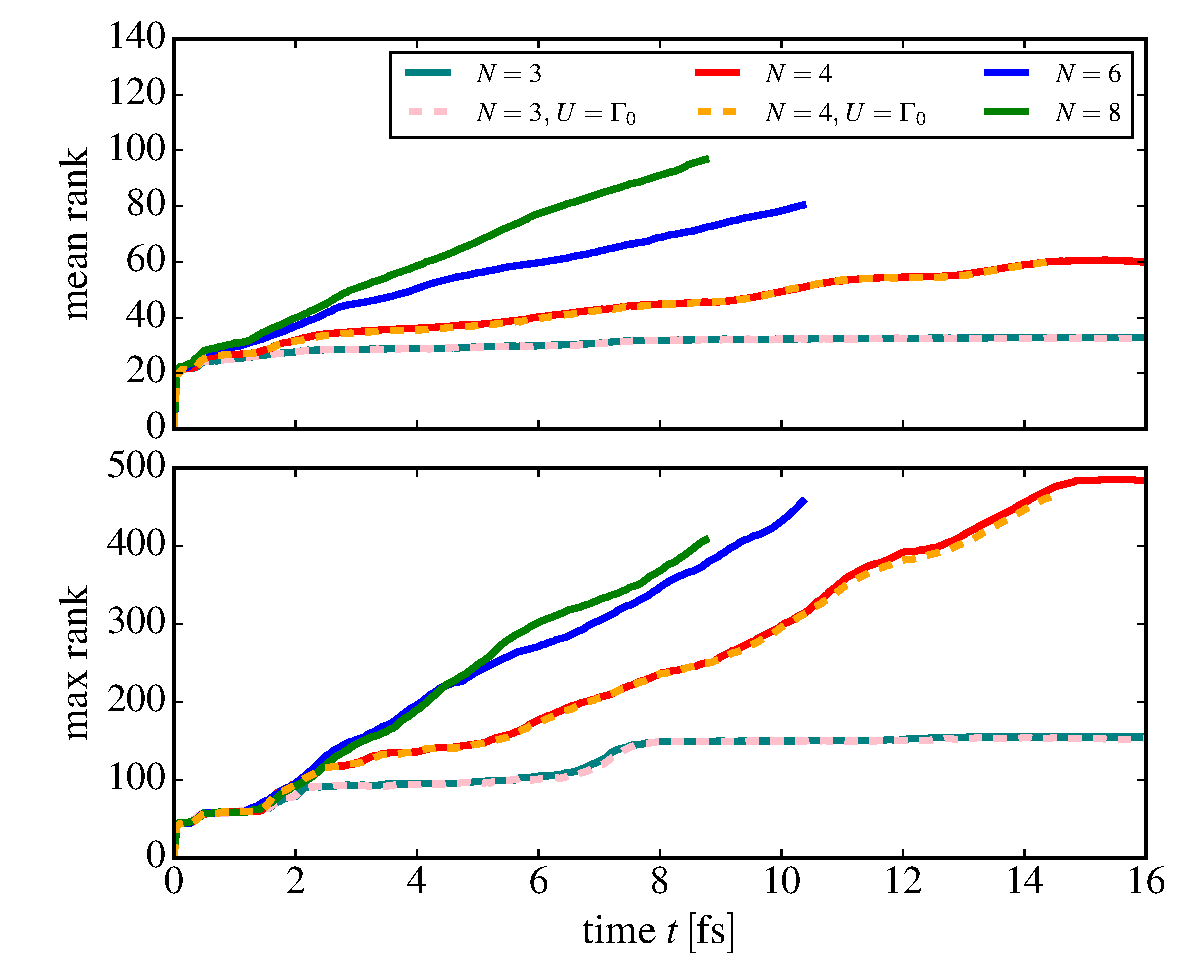
\includegraphics[width=0.8\textwidth]{figs/tamen_LVar_ranks.pdf}
	\caption{Full lines show the ranks for $U=0$.}
\end{figure}
\printbibliography
\end{document}


